\chapter{Background}
\label{chapter:background} 


\section{Datastores: from SQL to NoSQL systems}

A \textit{database} is an organized collection of data items, which are records of some real world information \cite{gray1993transaction}. Databases have always been extremely important in our society, from time ago with non-digital databases to nowadays with digital ones. They are a ubiquitous part of today's computing environment. 
\par
These database systems follow some data model, whose purpose is to determinate the logical structure of data items and how they are stored, organized and manipulated in data structures. As a vastly used data model we can found the relational model, used in SQL-based databases. 
\par
This data with its data model needs an structure to rely on, and this is called \textit{Database Management System} (DBMS). A DBMS is a suite of computer software programs that provides an interface between users and a database. They define mechanisms to build, store, maintain and modify one or more databases. 
DBMSes support any kind of applications, from business to Internet applications. They are one of the most important parts of many organizations and run critical applications that hospitals, airlines, banks and other types of organizations rely on for their daily operations.
\par
A relational database is a database which uses the relational model as its data model \cite{codd2001relational}. Its DBMS receives the name of Relational Database Management System (RDBMS) and it is the most popular example of database model. Most RDBMSes employ the SQL data definition and query language.
\par
Over the last three decades, RDMBSes have been the main technology for storing structured data. Even nowadays, the most popular DBMS continues being relational DBMS \cite{DBEnginesRanking}. RDMBS have been proved to be a good solution and have been evolved to fit new application requirements. These relational datastores have been and continue to be widely used. But with the amazing increase of generated data (Big Data), companies have seen how their needs have changed and they can not be addressed using the existing RDBMS technology, which have lead to the emergence of new datastores called NoSQL datastores, which are non-relational databases \cite{strauch2011nosql}.
\par
A NoSQL database is a database that uses less restricted data models than traditional relational databases, often loosing the ability to provide full ACID guarantees. Its main goals are its simplicity of design, horizontal scaling and higher availability. NoSQL systems are also revered to as "Not only SQL" due to some of them allow SQL-like query language.
\par
NoSQL is a term coined by Carlo Strozzi in 1998 to refer to an open-source relational database that did not use SQL \cite{Strozzi}. One year after, in 2009, the first NoSQL meet-up took placed in San Francisco. Computerworld magazine was there and stated in their article "No to SQL? Anti-database movement gains steam" that "NoSQLers came to share how they had overthrown the tyranny of slow, expensive relational databases in favor of more efficient and cheaper ways of managing data." \cite{ComputerworldNoSQL}. It evidents that new Web 2.0 Startups have started to use NoSQL datastores in order to handle the huge amounts of data the have to face instead the traditional RDBMS like MySQL \nocite{MySQL}, highly used in the startup environment before.
\par
In the last years, a great number of companies and projects have switched from relational towards non-relational datastores (NoSQL). By way of example, we find Cassandra \cite{ApacheCassandra}, developed at and used by Facebook, it is also used by Twitter \footnote{Cassandra at Twitter Today - https://blog.twitter.com/2010/cassandra-twitter-today} and Digg \footnote{Looking to the future with Cassandra - Http://about.digg.com/blog/looking-future-cassandra}, Projet Voldemort developed and employed at LinkedIn \footnote{Project Voldemort: Scaling Simple Storage at LinkedIn - http://blog.linkedin.com/2009/03/20/project-voldemort-scaling-simple-storage-at-linkedin/}, or the cloud NoSQL datastore Amazon SimpleDB \footnote{Amazon SimpleDB. -
http://aws.amazon.com/simpledb/} employed by Amazon.
\par
In order to realize how important the NoSQL environment is becoming , just a glance to the companies that are the pioneers or are in the cutting edge of the NoSQL movement is needed. They are enterprises running gigantic websites such as Google, Amazon, Twitter and Facebook, and others in the same field that use NoSQL datastores but modified to fit with their requirements due to their smaller scale.
\par



\subsection{The basic principles of NoSQL}
Three elements make up the basic pillars of the NoSQL datastores. They are the CAP theorem, the BASE theorem and the Consistency model. \cite{wang2012nosql}. These items are detailed in the following paragraphs.
\par
\begin{itemize}

\item CAP:
 In order to understand the design of NoSQL datastores, we must understand  the CAP theorem, introduced by Eric Brewer in 2000 \cite{CAP} and proved by Gilbert and Lynch \cite{ProbeCAP} in 2002. This theorem states that within a distributed data store, there are three properties that have a relationship of dependency, which are Consistency, Availability and Partition Tolerance.
\begin{itemize}
\item \textbf{Consistency} stands for clients must see always the same data.
\item \textbf{Availability} means each read or write request receives a response whether it was successful or failed.
\item \textbf{Partition Tolerance} means everything works despite physical networks partitions, except in case of total network failure. A network is partitioned when message losses occur between any two nodes of the system.
\end{itemize}

The CAP theorem affirms that a distributed data store can only satisfy at most two of these three conditions. Indeed, distributed systems like Cloud datastores, must allow Partition tolerance, otherwise they would be non-distributed systems. Therefore, this leaves us with only two real options to choose from: Consistency and Availability. Figure 2.1 depicts the CAP theorem's affirmation, only two out of the three properties share a segment, so that only two of them can be chosen at once.

\begin{figure}[htb]
\centering
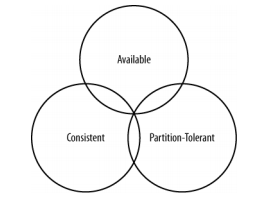
\includegraphics[width=0.5\textwidth]{./images/CAP.png}
\caption{The CAP theorem.} \label{fig:CAP}
\end{figure}

\par
According to this theorem, there are three possible views to design datastores, they are CA (primarily support Consistency and Availability), AP (primarily support Availability and Partition tolerance) and CP (primarily support Consistency and Partition tolerance).
\par
Figure 2.2 shows a graphical description of where each of the most relevant NoSQL and SQL solutions fit on the CAP continuum. The graphic was inspired by Dwight Merriman, CEO and founder of MongoDB, and updated by Eben Hewitt, Apache Cassandra Project Chair.
\begin{figure}[htb]
\centering
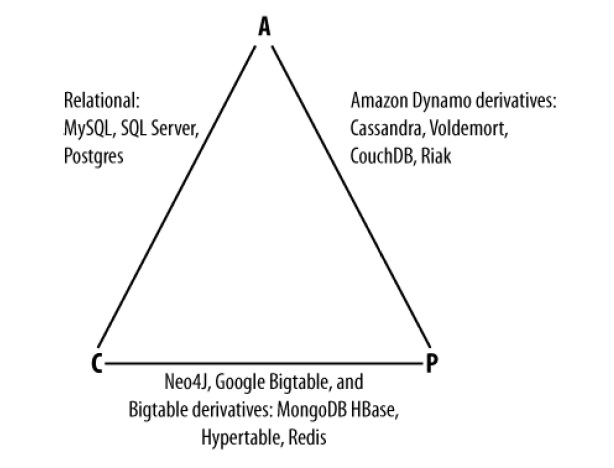
\includegraphics[width=0.6\textwidth]{./images/cap-examples.png}
\caption{CA, CP, AP real solutions.} \label{fig:CAP-examples}
\end{figure}

\par
As a brief summary, we can settle that traditional RDBMSes take Consistency and Availability but not Partition Tolerance. On the other hand, these new Cloud datastores, such as BigTable or Amazon Dynamo, take Partition Tolerance as we stated before, throwing away either Availability or Consistency respectively. 

\item BASE: 
ACID (Atomicity, Consistency, Isolation and Durability) datastores (traditional RDBMSes) are less powerful for distributed systems as they focus on strong consistency for transactions setting aside availability. Thus, it brings up a new softer consistency model widely adopted between most of the NoSQL datastores, which is: BASE \cite{pritchett2008base}, an acronym for Basically Available Soft-state services with Eventual-consistency. Basically available means partition failed could be supported, soft state indicates that the system could be non-synchronous sometimes and eventual-consistent implies that the data should be consistent after a reasonable time span. BASE can be seen as the opposite to ACID, while ACID requires the strongest consistency, BASE accepts eventually consistency, achieves availability and leads to levels of scalability that can not be obtained by any other way.

\fixme{figura del marcador de firefox, el qe sale ejes x e y, y como acid o base y manchas verdes.}

\item Consistency:
\textit{Consistency} is a datastore feature that has brought lot of controversy. As we have stated before, in the domain of Cloud datastores, trade-offs between consistency and availability (also referred to as latency in new CAP studies \cite{abadi2012consistency}) have been studied and done \cite{brewer2012cap} \cite{gilbert2012perspectives}. Consistency is divided in two sides: the client-side and the server-side. Client-side consistency refers to how and when users see updates made to an object in the storage system. There are three types, which are \cite{vogels2009eventually}:
\begin{itemize}
 \item \textbf{Strong consistency}, which means reading always returns the most recent written value.
\item \textbf{Eventual consistency}, which essentially means that all updates will propagate through-out all of the replicas in a distributed system, but this may take some time. Thus, all replicas will eventually converge to the same value, achieving strict consistency. 
\item \textbf{Weak consistency}, which stands for zero guarantees that subsequent access will return the updated value. The term \textit{inconsistency window} is used to refer to the period between the update and the moment when any user will see the updated value.
\end{itemize}

There are lots of eventual consistency levels \cite{wiki:consistency}, but they are out of the scope of this study.
\par
On the server side, consistency refers to how updates are done through the system and what guarantees the system gives with respect to updates. Here the consistency level can be modified, it can be tweaked from weak/eventual to strong consistency by playing with the number of replicas of the data that are contacted \cite{vogels2009eventually}.
\par
This "no total consistency" term has caused some uproar in the industry because as they argue, data is the heart of their business. But then why most popular web applications such as Amazon, Facebook or Twitter are using it. It is because companies have to choose between giving clients their results within a decent response time, or wait tons of minutes to get perfect consistent data. Nevertheless, it is worth mentioning that not all NoSQL datastores throw away consistency following strictly the scope of the BASE model, as we have explained, some NoSQL solutions offer degrees of consistency or even total by doing some trade-offs \cite{chang2008bigtable} \cite{cooper2008pnuts} \cite{ApacheHBase}.
\par
As an example, BigTable and HBase are strongly consistent (althought not fully ACID compliant) while Cassandra meets the eventual consistency and offers degrees of it.
\end{itemize}

After understanding the basic principles of NoSQL solutions, now we show the common key features these systems present.

\subsection{Key features of NoSQL Datastores}

Besides the three explained NoSQL pillars, Rick Cattell states in a 2010 SIGMOD paper \cite{cattell2011scalable} that NoSQL systems generally have six key features:
\begin{itemize}
\item The ability to horizontally scale "simple operation" throughput over many servers. ("simple operations" stands for key lookups, reads and writes of one or small number of records). In NoSQL datastores, query operations are simpler and easier than relational Joins or other complex SQL queries.

\item The ability to replicate and to partition data across servers based on a shared-nothing approach.

\item Clear and understandable interface to communicate with rather than SQL binding as in most relational databases.

\item Do not support ACID transactions in contrast to most relational databases. Instead they offer BASE (Basically, Available, Soft state, Eventually consistent), a softer concurrency model.

\item Efficient use of distributed indexes and RAM for data storage

\item Schemaless, which means users can add new attributes to data records at any time.

\end{itemize}


\subsection{Types of NoSQL Datastores}

Many of the organizations that have adopted NoSQL solutions to support their projects deal with massive amounts of unstructured or semi-structured data that does not fit anymore with the traditional fixed SQL data models. Each commented type of data features different characteristics, whereby each one requires different approaches to tackle it, which has turned out in different types of NoSQL solutions.
\par
According to the approach outlined by Rabi Prasad Padhy in a 2011 International Journal of Advanced Engineering Sciences and Technologies (IJAEST) paper \cite{padhy2011rdbms}, on a basic level, there are three main types of NoSQL datastores according to their data model:
\begin{itemize}
\item Key/value stores: Data is stored as key-value pairs; key is used as an index to find its value. These datastores can hold structured and unstructured data. Query operations are limited as the internal structure of data is not known. Some examples are Amazon's SimpleDB, Riak, Redis, Azure, GT.m, MemcachedDB and Voldemort.
\item Column-oriented Databases: Instead of sets of data in a structured table of columns and rows as in relational databases, Column-oriented databases contain one extendable column of related data. Examples of ColumnFamily databases are Google BigTable, Cassandra, HBase, HyperTable and OpenNeptune.
\item Document-based stores: These systems store indexed documents, as just defined. Documents hold data in a standard format such as JavaScript Object Notation (JSON). Users can add whatever they need to a document. The elements of a document can be arbitrarily complex and can be queried. Document databases are Apache CouchDB, MongoDB and Raven.
\end{itemize}



